%\RequirePackage{plautopatch} % パッチを自動的に適用してくれる

% 仕様 ----------------------------------------------------------------------------------------------------------------

\documentclass[b5paper,11pt,dvipdfmx]{jsarticle}
\usepackage{amsmath,amssymb,amsthm,amsfonts}
\usepackage{hyperref}
\usepackage{mathtools}
\usepackage{graphicx}
\usepackage{url}
\usepackage{calligra}
\usepackage{physics}
\usepackage{tikz}
\usepackage{tcolorbox}
\usepackage{mathcomp}
\usepackage{textcomp}
\usepackage{pxjahyper}

\numberwithin{equation}{section}
\theoremstyle{definition}
\newtheorem{thm}{定理}[section]
\newtheorem{lem}[thm]{補題}
\newtheorem{prop}[thm]{命題}
\newtheorem{cor}[thm]{系}
\newtheorem{ass}[thm]{仮定}
\newtheorem{conj}[thm]{予想}
\newtheorem{dfn}[thm]{定義}
\newtheorem{rem}[thm]{注}


% 追加するパッケージたち ----------------------------------------------------------------------------------------------------------------

\usepackage{mathrsfs} % 花文字をいれる
\usepackage{bm,ascmac,latexsym,color}
\usepackage{varwidth}
\usepackage{pxrubrica}
\usepackage{titlesec}
\usepackage{tocloft}
\hypersetup{
    colorlinks=true,
    %linkcolor=red,
    citecolor=red,
    %urlcolor=magenta
    }

\usetikzlibrary{calc}
\tcbuselibrary{raster,breakable,theorems,skins}


% プリアンブルおわり ==============================================================

\begin{document}

\title{ホログラフィック超伝導の進展から}
\author{oreo}
\date{}

\maketitle

%\tableofcontents

\begin{abstract}
    本記事ではホログラフィー原理による超伝導現象の解析の試みと,特にその近年の進展について紹介します.
    ホログラフィー原理とは重力理論とゲージ理論が等価であるという主張であり,
    量子重力理論の構築への足がけとして期待されている枠組みです.
    そんな熱い期待\footnote{筆者の主観です.}がかけられているホログラフィー原理は,実はその端緒を弦理論にもちます.
    にもかかわらず弦理論がよく言われる検証不可能性
    \footnote{弦理論の典型的なエネルギースケールは$10^{19}$GeV程度であり,
    現在稼働している加速器のエネルギースケールは$10^4$GeV程度です.
    かなりの差がありますね.この事実をもってして弦理論は現実的な観点から検証不可能であると言われたりすることがあります.
    ただ高エネルギースケールの弦理論から示唆される結果は,
    弦理論それ自体の検証ができなくとも我々がよく知っている現実的なスケールの物理も含んでいると期待しているわけですから,
    それら低エネルギー有効理論に対する制限を与えるなど多くの場面で有用です.
    ホログラフィー原理もその一種だと筆者は思っています.
    またstring phenomenologyという分野もあると聞きますが,筆者はその有用性と詳細を知らないのでこれには言及しません.}
    にとらわれず,実際に現実の観測量と結びつける研究が多数行われています.
    よく挙げられる例としてはクォーク・グルーオン・プラズマ\cite{Policastro01,Kovtun04}
    や超伝導\cite{Hartnoll08a,Hartnoll08b}があります.
    特に超伝導に関しては近年大きな発展があり,
    ホットトピックと言えると思います\footnote{筆者の主観です.},
    ということで今回は超伝導(正確には超伝導っぽいもの)のホログラフィー原理を用いた解析を見ていきましょう.
\end{abstract}


\section{ホログラフィー原理}
皆さんはホログラフィー原理,もしくはAdS/CFT対応という言葉を聞いたことがあるでしょうか?
AdS/CFT対応ともよばれ,$d + 2$次元の重力理論と$d + 1$次元のゲージ理論が等価になるという主張です.
これは光学における2次元平板に3次元像の情報が埋め込まれているホログラムにちなみこう呼ばれています.
1997年にMaldacenaにより最初の例\cite{Maldacena97}が示され,
以降多くの論文が弦理論の主戦場であるhep-thに限らず様々な分野で投稿されています.
ここではそのホログラフィー原理に関して簡単に概観していこうと思います
\footnote{ページ数と筆者の力不足によりほとんどお話になっています.
真面目に議論と計算を追うなら\cite{Witten98,Aharony99,Bousso02,Ammon15}あたりを参照してください.}.

ホログラフィー原理とはバルクと呼ばれる$d + 2$次元の反de Sitter(AdS)時空
\footnote{AdS時空とは,負の定曲率を持つアインシュタイン方程式の真空解です.
一方で我々の宇宙は$0$より少し大きい曲率をもつと考えられています.}
上の重力理論が,その時空の境界にある$d + 1$次元の共形場理論(CFT)
\footnote{共形場理論とは,スケール変換に対して対称性をもつ場の量子論のことです.
素粒子物理学だけでなく,物性物理学における相転移など様々な場面に現れる普遍的な理論です.}
と等価であるという主張です.
この対応の強力な点は,対応する2つの理論の結合の強さが逆転する点にあります.
境界の場の量子論が計算が非常に難しい強結合の状態にあるとき,
バルクの重力理論は,我々がよく知っている弱結合(つまり古典重力)の状態に対応します.
つまり我々がこれまで歯が立たなかった強結合な量子多体系の問題を,
より簡単な一般相対性理論の計算に「翻訳」して解くことができます
\footnote{量子重力理論の構築に向けた研究ではこの関係を逆に使い,
重力が十分強いときの重力理論を弱結合の場の量子論を使って解析します.}.
ホログラフィー原理に対する証明はないものの,多くの例が計算して確かめられており,
hep-thの文脈ではいくぶん信じられている推測だと思います.

ここで理論が等価であることの意味を具体的に述べておくと,
これは2つの理論における分配関数が一致していることを指します.
具体的にはよくGKP--Witten関係式\cite{Gubser98,Witten98}
\begin{equation}
    \exp(i S_{\text{tot}}[J])
    = \ev{\exp\left[ i \left( S_{\text{YM}}
    + \int \dd^{d+1} x \left. J \right|_{\text{boundary}} (x) \mathcal{O}(x) \right)\right]}
\end{equation}
が使われ,2つの理論の物理量を結びつけます
\footnote{ホログラフィー原理やGKP--Wittenのような関係式は超弦理論における閉弦と開弦の間にある双対性から示唆されます.
弦理論はその名の通り,1次元の自由度をもつ弦を基本的対象とする理論のことで,
0次元の質点からなる従来の素粒子理論から自由度が増えている分,様々なことを表現できるようになります.
素粒子物理学における一つの目的はすべての事象を説明するような統一理論の構築にありますが,
現状の理論では4つある基本相互作用のうち重力とそれ以外の相互作用についての理論を
うまく整合して組み合わせることができていません.
これは重力の量子化がこれまでの手法ではうまくいかないことに起因します.
(ここではこれ以上触れませんが,歴史を含めたこれに関する話題は\cite{Yoneya21}が詳しいと思います.)
現在明確な実験事実等はないものの,これを解決する統一理論として超弦理論は期待されています.
ということは我々の知っている物理は弦理論に低エネルギー有効理論として含まれているはずです.
弦理論の基本構成要素である弦には両端がつながっている閉弦と両端がつながっていない開弦があり,
これらの低エネルギー有効理論はそれぞれ重力理論とゲージ理論です.
そして閉弦と開弦はDブレーンという対象を通じて等価な物理を見ていると考えられており,
ここから低エネルギー有効理論どうしの対応関係が示唆されます.}.
バルク中の場$\mathcal{J}(x)$が境界上の物理量$\mathcal{O}(x)$のソースとなって対応しています.
\begin{figure}[t]
    \centering
    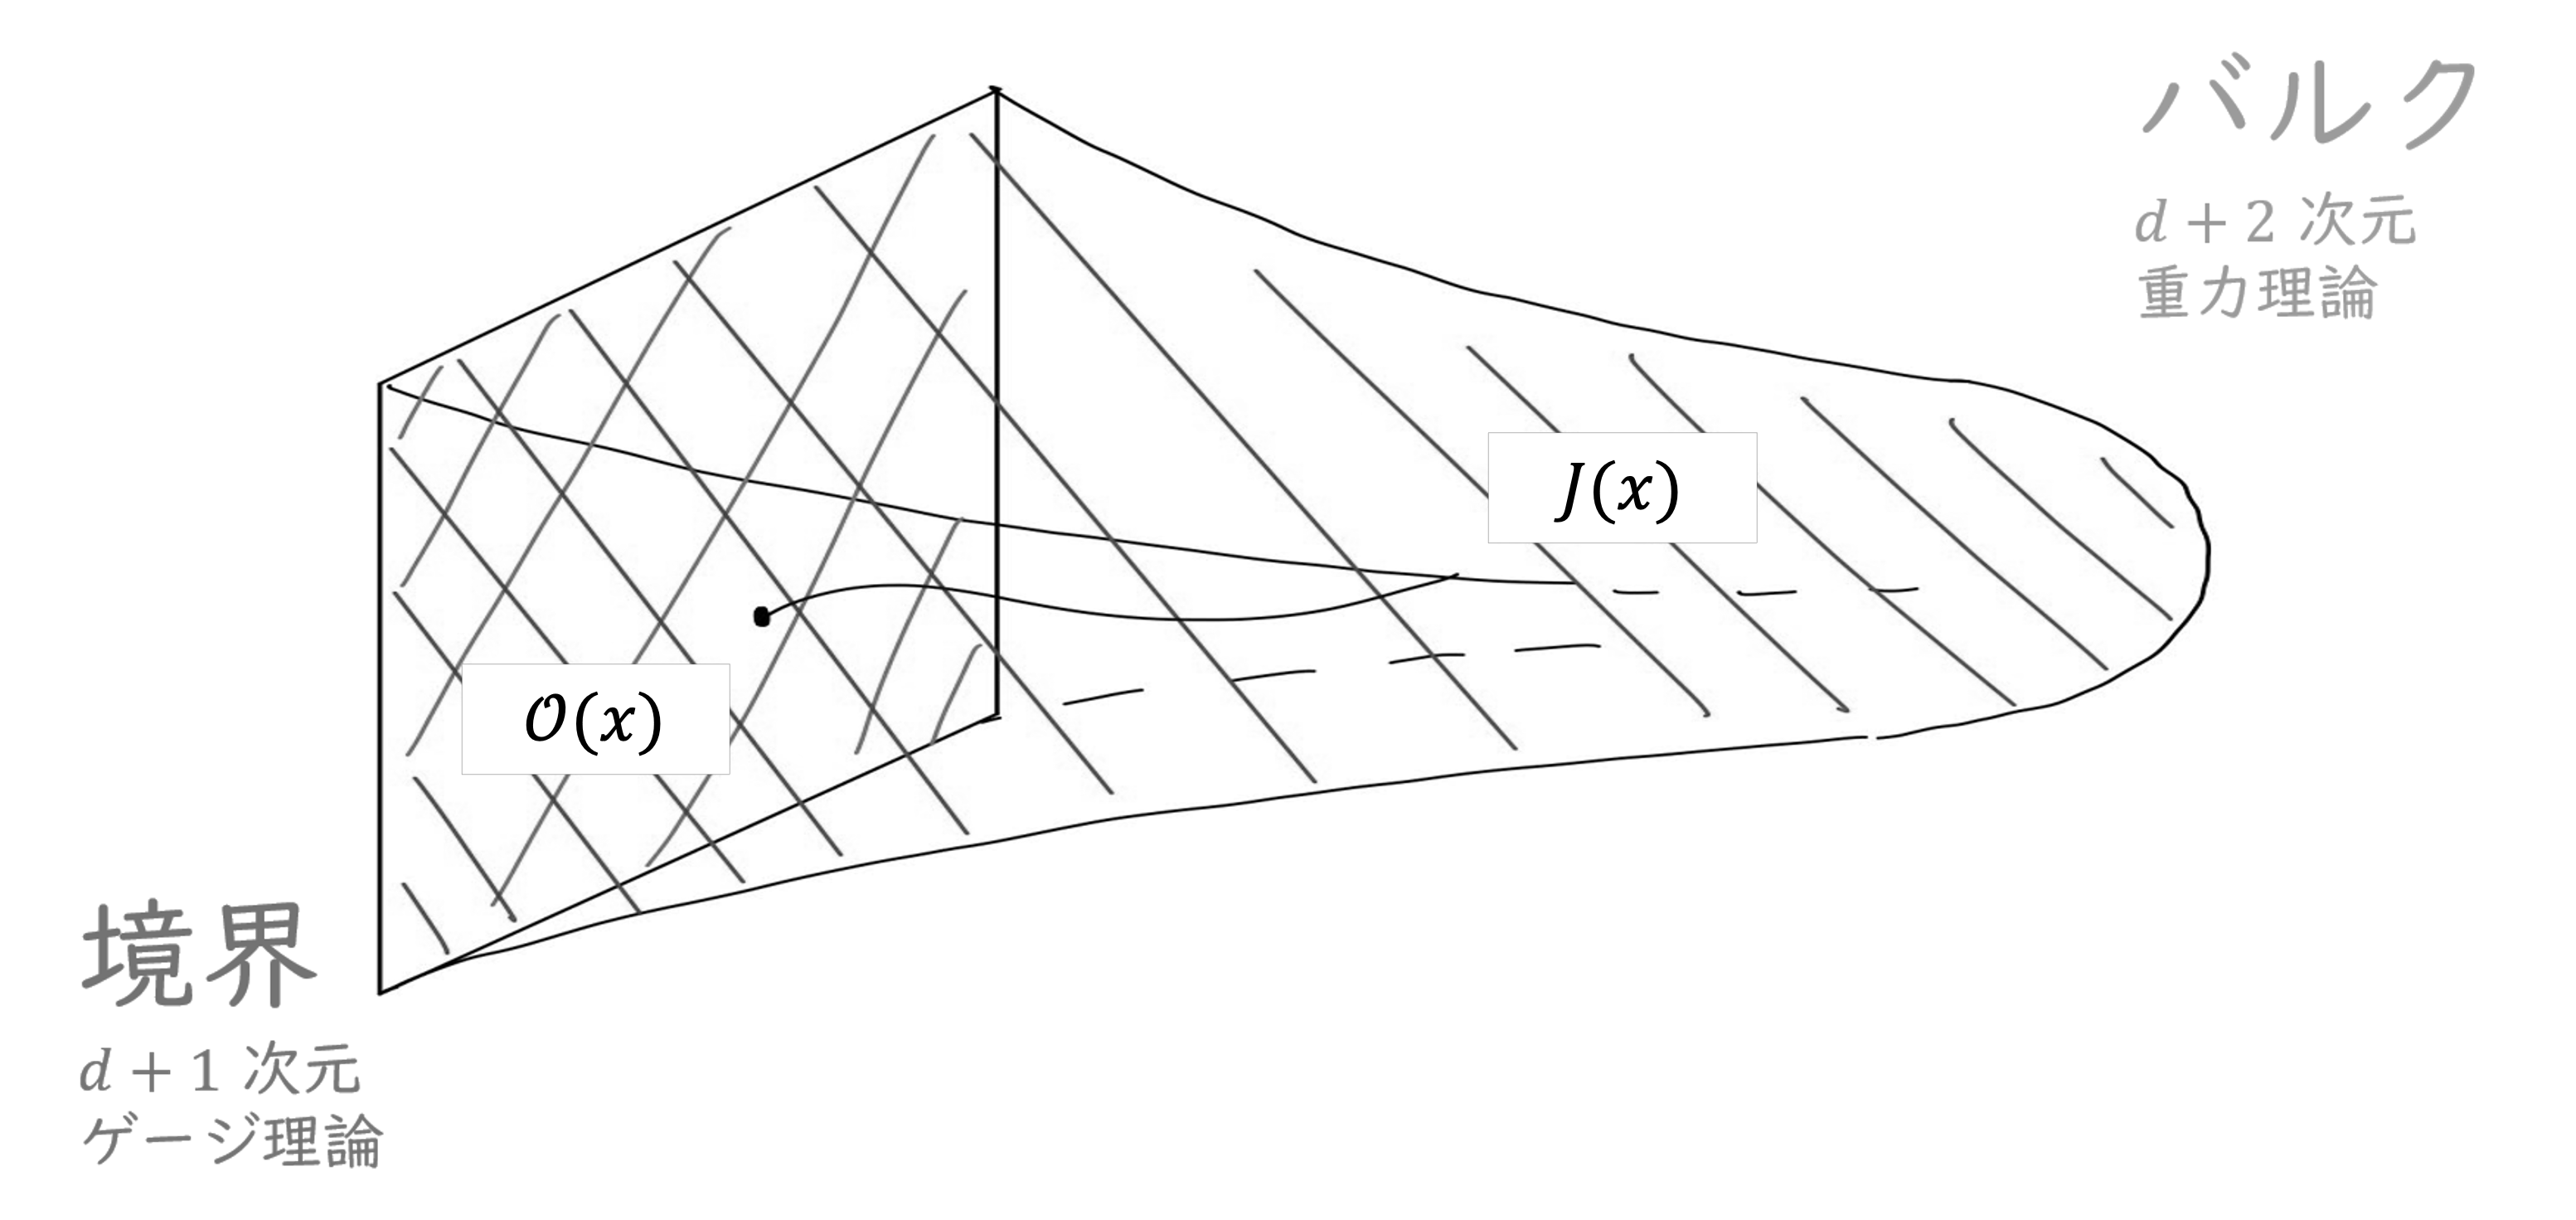
\includegraphics[width=0.7\textwidth]{fig_kawai/holography_bw.png}
    \caption{ホログラフィー原理の概念図.
    バルクの重力理論が境界の場の量子論と等価になる.
    その際,バルクにおける場が境界上の物理量に対するソースとして対応する.}
    \label{fig:holography}
\end{figure}


\subsection{具体例:クォーク・グルーオン・プラズマ}
ここでホログラフィー原理が話題になる契機となった代表的な例の話をしておきましょう.
Brookhaven National Laboratoryが開発したRelativistic Heavy Ion Colliderという加速器があります.
この中ではすごい速さで重イオン同士をぶつけるという実験がされており,
その目的はクォーク・グルーオン・プラズマ(QGP)の生成とその性質の解析です.
QGPとは陽子や中性子の中にある,普段単体で外には出てこないクォークが
高温高圧化では単体で自由に動けるようになった状態です.
クォークを基本自由度とする理論から見るとこれは強結合になっていて,解析が困難です.
そのためこの実験で実際に生成される以前はQGPの振る舞いが
理想気体に近いのか,それとも完全流体に近いのかはっきりしませんでした.
そんな中ホログラフィーを用いた弦理論による計算ではQGPは完全流体であると予想されていました\cite{Policastro01,Kovtun04}.
そして実験結果では実際に完全流体に近しい振る舞いをすると報告されています\cite{PHENIX06}.
実際にその実験レポートでは粘性の「予言」が整合しているとしてホログラフィー原理,
もとい超弦理論の論文\cite{Kovtun04}を引用しています.
\begin{description}
    \item[実験結果] $\frac{\eta}{s} \approx 0.1$,
    \item[ホログラフィーによる計算] $\frac{\eta}{s} = \frac{1 \hbar}{4 \pi k_B} \approx 0.08$.
\end{description}
これは実験検証から程遠いとされていた弦理論にとって驚きの結果と言えます.
このようにクォーク・グルーオン・プラズマにおける「成功」があり,
他の例への応用もより精力的に研究されるようになりました.
その一例が今回紹介する超伝導です.


\section{ホログラフィック超伝導}
以降ではまずは強結合量子多体系の一例としてホログラフィーで再現することになる,高温超伝導自体の説明をしたあと,
ホログラフィック超伝導の走りとなるHartnollらによる模型\cite{Hartnoll08a,Hartnoll08b}を説明します.
そして最後に,近年の進展として夏梅らによる模型\cite{Natsuume22}を紹介します.

\subsection{高温超伝導について軽く}
皆さんご存知の通り超伝導は普段は有限の値となる電流や熱流に対する抵抗値が温度以下でゼロとなる現象のことであり,
MRIなどの医療や加速器などの科学実験など様々な場面で活用されています.
ただし高温状況下ではもちろんのこと,高磁場下でもその特性は失われるなど,
産業規模で超伝導を利用するにはいくつかの障壁があります.
ただ積み重なる研究により,銅酸化物超伝導体などをはじめとする高温超伝導体が発見され,
これらは100K程度の高温下でも超伝導状態を維持します.
\begin{figure}[t]
    \centering
    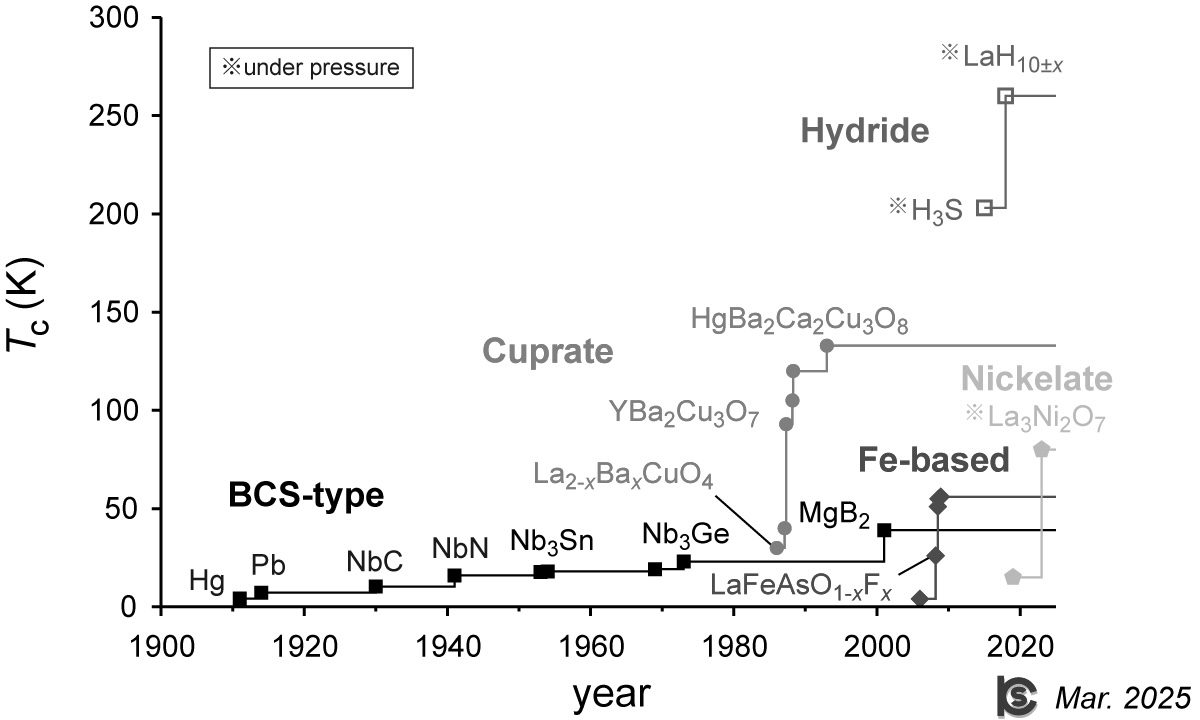
\includegraphics[width=0.7\textwidth]{fig_kawai/tc-history_2025_bw.jpg}
    \caption{超伝導転移温度の記録 【引用】東京大学 大学院総合文化研究科 広域科学専攻 相関基礎科学系 橘高研究室 [\url{https://park.itc.u-tokyo.ac.jp/kittaka/contents/others/tc-history/index.html}]}
    \label{fig:tc-history}
\end{figure}
一方で高温超伝導を理論的な側面から見ると,いまだその機構は不明であり,難問となっています.
従来型の超伝導の機構を説明する模型としてBCS理論が有名です.
格子振動により電子間に有効的な引力が働き電子2つが対となることでボース粒子のキャリアが生まれる,
このようにBCS理論は超伝導のゼロ抵抗を説明していますが,
40Kを超えたあたりで格子振動が激しくなるため,この描像は成り立たないことが知られています.
こうなると他の機構を考えるしかないわけですが,電子同士が対になって凝縮するわけですから,
電子電子間相互作用をそこそこ真面目に考えてやる必要が出てきます.
これが高温超伝導の強結合の部分です.
ホログラフィック超伝導は強結合で解析が難しいとされる高温超伝導を簡単に計算できうる希望を持っています.


\subsection{模型の構築}
ということでホログラフィー原理を利用して超伝導を再現するような模型を作りましょう.
ただし高温超伝導を直接的に記述するゲージ場の理論を我々は知らないので,
理論全体で超伝導っぽい振る舞いをするようなものを構築します.
用意するのはこちらです.
\begin{description}
    \item[有限温度系] ブラックホール解
    \item[電荷保存則] Maxwell場$A_M$
    \item[電子対生成] 複素スカラー場$\Psi$
\end{description}
説明していきます.
ホログラフィーとは重力理論とゲージ理論が等価であり,バルクの場と境界の物理量が一対一に対応しているのでした.
境界の理論は,高温超伝導に類似した性質を持つわけですから,
有限温度系であり,電流(カレント)をもち,超伝導転移(2次相転移)を起こすことが期待されます.
ホログラフィーにおいて有限温度の系を再現する際に用いるのはブラックホールです.
これはブラックホール自体が温度をもつ有限温度系であるためです.
重力理論側の計量をブラックホール解にしておくことでHawking温度をもつ有限温度系とみなせます.
また,カレント$\mathcal{J}^\mu$を生成するソースが必要となります.これはMaxwell場$A_M$でいいでしょう.
最後に相転移を起こすために秩序変数$\ev{\mathcal{O}}$を導入してやりましょう.
これに結合する場として複素スカラー場$\Psi$を導入します.
するとバルクが$d+2$次元時空中のアインシュタイン・マクスウェル・スカラー理論
\begin{equation}
    \begin{split}
        S_{\text{bulk}}
        &= \int \dd^{d+2} x \sqrt{-g} \left( \mathcal{L}_g + \mathcal{L}_{\text{matter}} \right)\\
        \mathcal{L}_{g}
        &= R - 2 \Lambda\\
        \mathcal{L}_{\text{matter}}
        &= - \frac{1}{g^2} \left( \frac{1}{4} F^{MN} F_{MN} + |D_M \Psi|^2 + m^2 |\Psi|^2 \right)
    \end{split}
\end{equation}
ただし
\begin{equation}
    \begin{split}
        F_{MN} &= \partial_M A_N - \partial_N A_M,\\
        D_M &= \nabla_M - i A_M,\\
        \Lambda &= - \frac{3}{L^2}
    \end{split}
\end{equation}
でかけることになります.
これはホログラフィック超伝導体を記述する標準的なモデルです.
以降はバルクが$(3+1)$次元の模型を考えます.
このままでは重力場がいくつかの物質場と結合していて,解析が難しそうなので,
こういった場合はよくプローブ極限($g \gg 1$)をとってやって物質場からの寄与を無視します.
するとバルクの背景時空としてSchwarzschild-AdS$_4$解を素直に入れることができます.
\begin{equation}
    \begin{split}
        \dd s_4
        &= r^2 (- f^2 \dd t^2 + \dd x^2 + \dd y^2) + \frac{\dd r^2}{r^2 f} \\
        &= \left(\frac{r_0}{u}\right)^2 (- f^2 \dd t^2 + \dd x^2 + \dd y^2) + \frac{\dd u^2}{u^2 f} \\
        f &= 1 - \left( \frac{r_0}{r} \right)^3 = 1 - u^3
    \end{split}
\end{equation}
このブラックホールのHawking温度$2 \pi T = \frac{3 r_0}{2 L^2}$が境界の$(2+1)$次元時空の温度に対応します.
AdS時空の半径$L$とホライズン半径$r_0$をそれぞれ1に固定して議論します.
このもとで各場についての運動方程式から漸近形を決定し,GKP--Wittenから境界上の物理量と対応づけるのですが,
諸事情\footnote{申告したページ数が少なすぎたようです.計算例は\cite{夏梅SGC}に載っています.}
により細かい計算は省略して書いていきます.
物質場の漸近的振る舞いは
\begin{equation}
    \begin{split}
        A_\mu &\sim \mathcal{A}_\mu+A_\mu^{(+)} u,\\
        \Psi &\sim \Psi^{(-)} u^{\Delta_{-}}+\Psi^{(+)} u^{\Delta_{+}},\\
        \Delta_{\pm} &\coloneq \frac{3}{2} \pm \nu, \quad \nu = \sqrt{\frac{9}{4}+m^2}.
    \end{split}
\end{equation}
とかけます.
ここでバルクのベクトルポテンシャル$A_\mu$の境界値が境界のベクトルポテンシャル$\mathcal{A}_\mu$,
$A_\mu$の次のオーダーの項$A_\mu^{(+)}$が境界の電流$\ev{\mathcal{J}_\mu}$に,
バルクのスカラー場$\Psi$の境界での主要項$\Psi^{(+)}$が超伝導の秩序パラメータ$\ev{\mathcal{O}}$,
$\Psi^{(-)}$がそのソースに対応します:
\begin{equation}
    \begin{split}
        \ev{\mathcal{J}_\mu} &= \left.\frac{1}{g^2} F_{u \mu}\right|_{u=0} \\
        \ev{\mathcal{O}} &=\frac{1}{g^2} 2 \nu \Psi^{(+)}.
    \end{split}
\end{equation}
\begin{figure}[t]
    \centering
    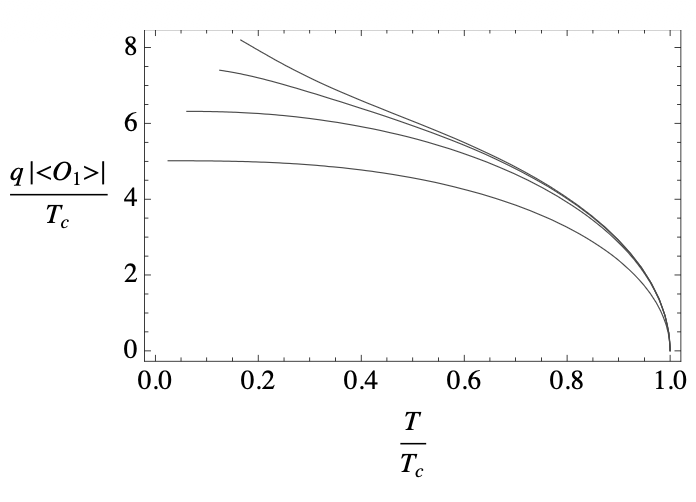
\includegraphics[width=0.7\textwidth]{fig_kawai/order_para.png}
    \caption{$\Psi(u)$の数値計算結果(\cite{Hartnoll08b}から引用)}
    \label{fig:order_para}
\end{figure}
図\ref{fig:order_para}からオーダーパラメータが転移温度近傍で
\begin{equation}
    \ev{\mathcal{O}} \propto (T_c - T)^{\frac{1}{2}}
\end{equation}
と振る舞うことがわかります.
どうも相転移は起きていそうです.


\subsection{より現実的なモデルにするために}
上で作った模型は現実の超伝導の解析という目的からすると多くの問題があります.
\begin{itemize}
    \item Meissner効果を確認していない
    \item 境界上の秩序変数$\ev{\mathcal{O}}$の微視的病像が不明である
    \item 対応する境界の理論がU(1)ゲージ理論ではなくラージ$N$ゲージ理論になっている
    \footnote{古典重力理論を使って解析しているために対応する理論はラージN極限と呼ばれる仮定がなされており,
    単純なU(1)ゲージ理論とは異なります.ただしここでは割愛して話を進めます.
    真っ当な電磁場を対象としているわけではないことだけ注意してください.}
\end{itemize}
ここでは一つ目のMeissner効果について考えましょう.
Meissner効果は超伝導であると断定するために必要な,超伝導体の重要な特徴です.
しかし従来のホログラフィック超伝導の模型ではDirichlet境界条件を課していいたため,境界でバルクのゲージ場が固定され,
境界上には動的なMaxwell場そのものは存在しません.
そこでMaxwell場のダイナミクスを回復してやるために,次のような新たな境界条件を考えましょう.
\begin{equation}
    \partial_{j} \mathcal{F}^{ij}
    = e^{2} \left( \ev{\mathcal{J}^{i}} + \mathcal{J}_{\text{ext}}^i \right)
\end{equation}
ここで,非自明な解をとるためにソース$\mathcal{J}_{\text{ext}}^i$を加えています.
これにフーリエ変換したゲージ場
\begin{equation}
    A_y = \int \frac{\dd q}{2 \pi} e^{iqx} \tilde{A}_y
\end{equation}
を入れて解きます.このもとで境界上のMaxwell場は
\begin{equation}
    q^2 \tilde{\mathcal{A}}_y
    = \frac{e^2}{1 + e^2} \tilde{\mathcal{J}}^{\text{ext}}_y
    \coloneq \mu_m \tilde{\mathcal{J}}^{\text{ext}}_y
\end{equation}
とかけて,透磁率がわかります.
帯磁率を求めて,あわせて温度に対応するホライズン半径を陽に描いてやると
\begin{equation}
    \begin{split}
            \mu_m
            &= \frac{e^2}{1 + e^2 / r_0}\\
            \chi_m
            &= - \frac{e^2 / r_0}{1 + e^2 / r_0}.
    \end{split}
\end{equation}
これは低温で完全反磁性になりますね.


\section{まとめと展望}
本記事ではホログラフィー原理を用いた超伝導の記述について,
その基礎的なモデルからMeissner効果を直接的に示す新規的な模型までを駆け足で紹介しました.
まず荷電ブラックホールに複素スカラー場を導入することで超伝導相転移が起きることを確認しました.
つぎに近年の夏梅と岡村による,ゲージ場のダイナミクスを回復するような境界条件を課して完全反磁性
つまりMeissner効果を解析的に導出し,より現実の超伝導体に近しい模型となりました.
これはホログラフィー原理が単なる概念的な対応関係に留まらず,
物性物理学の具体的な問題に対する強力な計算手段になりうる可能性をより強く知らしめる結果です.
もちろん,これらのモデルはまだ理想的な状況下での計算であり,
現実の高温超伝導体と比較するには,先述のように秩序変数$\ev{\mathcal{O}}$の微視的な描像や,
具体的に対応する境界のゲージ理論の実態など,多くの不明点が残されています.
しかし現状明確な理論的説明が与えられていない高温超伝導に対して,
ホログラフィーを通した簡単な模型構築によりいくつかの計算ができることは大きな利点であり,
その詳細がわかっていないホログラフィー原理と高温超伝導の両者に対する理解を深める上で重要な研究と言えるでしょう.

\begin{thebibliography}{99}
    \bibitem{Policastro01} G. Policastro, Dan T. Son, and Andrei O. Starinets. The Shear viscosity of strongly coupled N=4 supersymmetric Yang-Mills plasma. Phys. Rev. Lett., Vol. 87, p. 081601, 2001.
    \bibitem{Kovtun04} P. Kovtun, Dan T. Son, and Andrei O. Starinets. Viscosity in strongly interacting quantum field theories from black hole physics. Phys. Rev. Lett., Vol. 94, p. 111601, 2005.
    \bibitem{Hartnoll08a} Sean A. Hartnoll, Christopher P. Herzog, and Gary T. Horowitz. Building a Holographic Superconductor. Phys. Rev. Lett., Vol. 101, p. 031601, 2008.
    \bibitem{Hartnoll08b} Sean A. Hartnoll, Christopher P. Herzog, and Gary T. Horowitz. Holographic Superconductors. JHEP, Vol. 12, p. 015, 2008.
    \bibitem{Maldacena97} Juan Martin Maldacena. The Large N limit of superconformal field theories and supergravity. Adv. Theor. Math. Phys., Vol. 2, pp. 231–252, 1998.
    \bibitem{Witten98} Edward Witten. Anti de Sitter space and holography. Adv. Theor. Math. Phys., Vol. 2, pp. 253–291, 1998.
    \bibitem{Aharony99} Ofer Aharony, Steven S. Gubser, Juan Martin Maldacena, Hirosi Ooguri, and Yaron Oz. Large N field theories, string theory and gravity. Phys. Rept., Vol. 323, pp. 183–386, 2000.
    \bibitem{Bousso02} Raphael Bousso. The Holographic principle. Rev. Mod. Phys., Vol. 74, pp. 825–874, 2002.
    \bibitem{Ammon15} Martin Ammon and Johanna Erdmenger. Gauge/gravity duality: Foundations and applications. Cambridge University Press, Cambridge, 4 2015.
    \bibitem{Gubser98} S. S. Gubser, Igor R. Klebanov, and Alexander M. Polyakov. Gauge theory correlators from noncritical string theory. Phys. Lett. B, Vol. 428, pp. 105–114, 1998.
    \bibitem{Yoneya21} 民明米谷. 究極理論への道 : 力・時空・物質の起源を求めて. 岩波書店, 2021.
    \bibitem{PHENIX06} A. Adare, et al. Energy Loss and Flow of Heavy Quarks in Au+Au Collisions at s(NN)**(1/2) = 200-GeV. Phys. Rev. Lett., Vol. 98, p. 172301, 2007.
    \bibitem{Natsuume22} Makoto Natsuume and Takashi Okamura. Holographic meissner effect. Phys. Rev. D, Vol. 106, p. 086005, Oct 2022.
    \bibitem{夏梅SGC} 夏梅誠. 超弦理論の応用. SGC ライブラリ, No. 93. サイエンス社, 2012.
\end{thebibliography}

\end{document}